\chapter{String Art}

\begin{quote}
The artist is a receptacle for the emotions that come from all over
the place: from the sky, from the earth, from a scrap of paper, from a
passing shape, from a spider's web.

\hfill---Pablo Picasso
\end{quote}


\section{I'm Seeing Stars}\index{stars}

Can you remember when you first learned to draw a star? I can! I was first taught to draw a star like this:
\[
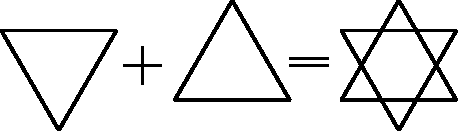
\includegraphics{../graphics/bartTri.pdf}
\]
But I wanted to know how to draw 5-pointed stars like the other
kids. So one day I taught myself to draw a star like this:
\[
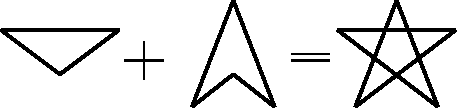
\includegraphics{../graphics/bartTri2.pdf}
\]
This may seem like a silly way to draw this star---it certainly makes
me chuckle now. Let's see if we can give a theory for drawing stars
that will connect the two different stars above, teach you how to
draw some new stars, and learn a little more mathematics along the
way.

We'll start with $5$ points equally spaced on a circle:
\[
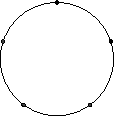
\includegraphics{../graphics/stfive.pdf}
\]
Think of these points as \textit{pins}.  Next we'll start at the top
and draw lines that we'll think of as \textit{strings}, moving
clockwise to the point two steps away each time:
\[
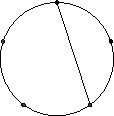
\includegraphics{../graphics/stfive1.pdf}\qquad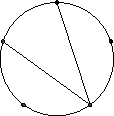
\includegraphics{../graphics/stfive2.pdf}\qquad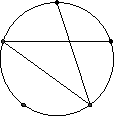
\includegraphics{../graphics/stfive3.pdf}\qquad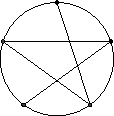
\includegraphics{../graphics/stfive4.pdf}\qquad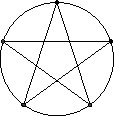
\includegraphics{../graphics/stfive5.pdf}
\]
Check it out, we got a star! If we had used pins and string to make
this star, we could have done it with one piece of string.

Now start with $6$ points equally spaced on a circle. Again, we'll
move clockwise two steps each time:
\[
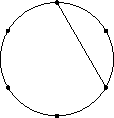
\includegraphics{../graphics/stsix1.pdf}\qquad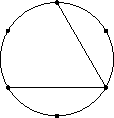
\includegraphics{../graphics/stsix2.pdf}\qquad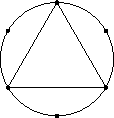
\includegraphics{../graphics/stsix3.pdf}
\]
Oops, we've run out of points! No worries, just start again at one of
the points that hasn't been touched by a line yet, drawing lines and
moving two steps each time:
\[
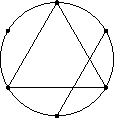
\includegraphics{../graphics/stsix4.pdf}\qquad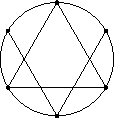
\includegraphics{../graphics/stsix5.pdf}\qquad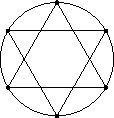
\includegraphics{../graphics/stsix6.pdf}
\]
Ah! The other star! In this case, if we used pins and strings, we'd
need to use \textit{two} pieces of string. Hmmm---at this point I have
a question:
\begin{ques} 
How do we actually draw $n$ equally spaced points on a circle?
\end{ques}
\QM 
You can figure that one out---or just ask someone who is standing up at
the front of some room talking to themselves. Oh! And I have another
question:
\begin{ques} 
What happens if you put $n$ points, and connect them by moving $s$
steps each time?
\end{ques}
I'm feeling generous, so I'll help out with this one. Let's do a bunch
of examples together. I'm hoping that the following notation will help
out:\index{ns@$\star{n}{s}$}
\[
\star{n}{s}=\text{the star with $n$ equally spaced points where we move $s$ steps clockwise}
\]
\begin{war}
Remember, $\star{n}{s}$ is a star, \textbf{not} a fraction!
\end{war}
Armed with our new notation, let's draw the following stars!
\[
{
\renewcommand{\arraystretch}{1.5}
\begin{array}{|c|c|c|}\hline
 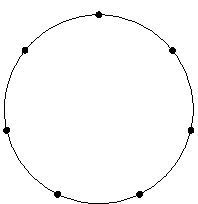
\includegraphics{../graphics/stseven.pdf} & 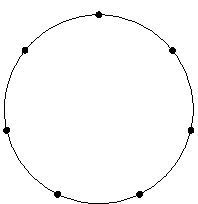
\includegraphics{../graphics/stseven.pdf} & 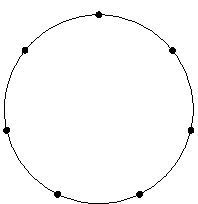
\includegraphics{../graphics/stseven.pdf} \\
\star{7}{1} & \star{7}{2} & \star{7}{3} \\\hline 
 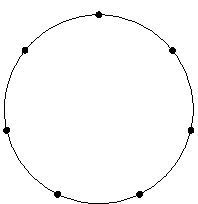
\includegraphics{../graphics/stseven.pdf} & 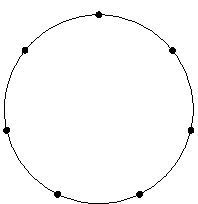
\includegraphics{../graphics/stseven.pdf} & 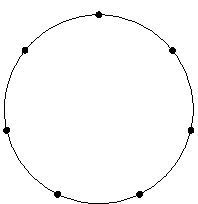
\includegraphics{../graphics/stseven.pdf} \\
\star{7}{4} & \star{7}{5} & \star{7}{6} \\\hline 
\end{array}
}
\]

\begin{ques}
Do you notice any patterns? Why not share your observations with a
friend---or an enemy?
\end{ques}
\QM

\begin{ques}
Looking back, we see that some stars, like $\star{7}{2}$, are one piece (or would use one piece of string). Other stars, like $\star{6}{2}$, are more than one piece. What's the general rule?
\end{ques}
\QM


\newpage


\problems
\begin{enumerate}
\item Explain what is meant by the symbol $\star{n}{s}$.
\item Explain how to draw $n$ equally spaced points on a circle.
\item Use a compass and protractor to draw $\star{3}{s}$ for $s =
  1,2$. Which of these look the same?  How many pieces are there in
  each case?
\item Use a compass and protractor to draw $\star{4}{s}$ for $s =
  1,2,3$. Which of these look the same? How many pieces are there in
  each case?
\item Use a compass and protractor to draw $\star{5}{s}$ for $s =
  1,2,3,4$. Which of these look the same? How many pieces are there in
  each case?
\item Use a compass and protractor to draw $\star{6}{s}$ for $s =
  1,2,3,4,5$. Which of these look the same? How many pieces are there
  in each case?
\item Use a compass and protractor to draw $\star{7}{s}$ for $s =
  1,\dots,6$. Which of these look the same? How many pieces are there
  in each case?
\item Use a compass and protractor to draw $\star{8}{s}$ for $s =
  1,\dots,7$. Which of these look the same? How many pieces are there
  in each case?
\item Use a compass and protractor to draw $\star{9}{s}$ for $s =
  1,\dots,8$. Which of these look the same? How many pieces are there
  in each case?
\item Fill in the following table by sketching the stars: 
\[
\begin{array}{|c||c|c|c|c|c|c|c|c|}\hline
n\backslash s & 1 & 2 & 3 & 4 & 5 & 6 & 7 & 8 \\ \hline\hline
3 & & & & & & & & \\ \hline
4 & & & & & & & & \\ \hline
5 & & & & & & & & \\ \hline
6 & & & & & & & & \\ \hline
7 & & & & & & & & \\ \hline
8 & & & & & & & & \\ \hline
\end{array}
\]
Your sketch must
be clear and show the distinguishing features of each star.
\item Give three different stars each made of 2 connected
  pieces. Explain your reasoning.
\item Give three different stars each made of 3 connected
  pieces. Explain your reasoning.
\item Give three different stars each made of 4 connected
  pieces. Explain your reasoning.
\item Give three different stars each made of 5 connected
  pieces. Explain your reasoning.
\item Draw $\star{7}{9}$, what happens? Explain why we never need to
  discuss the case $s\ge n$ when drawing $\star{n}{s}$.
\item Perceptive Persephone claims that $\star{5}{2}$ is \textit{not}
  equal to $\star{5}{3}$. They look the same to me! Please explain
  what is she going on about.
\item Give a precise description of when two stars $\star{n}{s}$ and
  $\star{n}{t}$ will look the same. Explain why your description
  holds.
\item Give a precise description based on $n$ of how many different-looking
 stars $\star{n}{s}$ can be formed. Explain why your
  description holds.
\item Give a precise description based on $n$ of when a star
  $\star{n}{s}$ is one piece for all values of $s$. Explain why your
  description holds.
\item Give a precise description based on $n$ and $s$ of when a star
  $\star{n}{s}$ is one piece. Explain why your description holds.
\item Explain how to figure out how many pieces a star $\star{n}{s}$
  will have \textit{without} drawing the star.
\item Give a precise description of what happens when we ``reduce to
  lowest terms.'' As an example, think about how the stars
  $\star{6}{2}$ and $\star{3}{1}$ are related. Explain why your
  description holds.
\item Draw $\star{4}{2}$, $\star{6}{3}$, and $\star{8}{4}$.  What do you
  notice? Let's call these stars \textit{asterisk stars}. Give a precise
  description of when you can draw asterisk stars---and when you cannot
  draw asterisk stars. Explain why your description holds.
\item Interested Isabel finds $\star{7}{2}$ and $\star{7}{3}$
  interesting. Why?
\item Interested Isabel finds $\star{10}{2}$ and $\star{10}{4}$
  interesting. Why?
\end{enumerate}

\newpage










\section{Drawing Curves}


\subsection{Envelope of Tangents}

Get out a piece of paper, a ruler, and a writing utensil. Really, do
it!  Seriously! Now draw two lines that come to a point:
\[
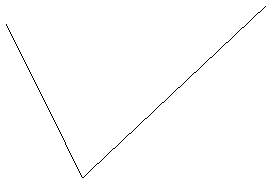
\includegraphics{../graphics/mesh0.pdf}
\]
Next, take both of those lines and mark the midpoints. Connect the
midpoints with a line:
\[
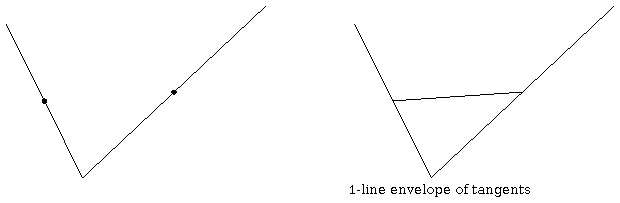
\includegraphics{../graphics/mesh1.pdf}
\]
Each original line is now divided into two segments. Mark the
midpoints of those segments and cross-connect them:
\[
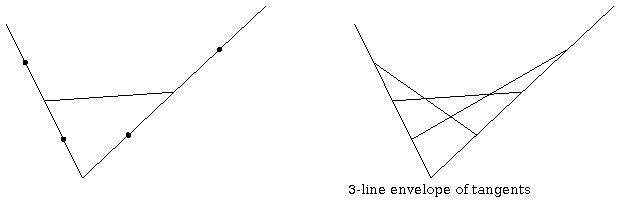
\includegraphics{../graphics/mesh2.pdf}
\]
If you continue this cross-connecting process, you'll get groovy pictures like these:
\[
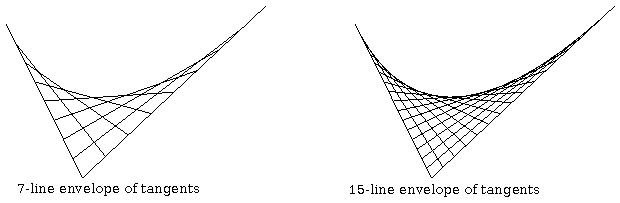
\includegraphics{../graphics/mesh3.pdf}
\]
Over 2000 years ago, Apollonius of Perga explained why the curve formed by these segments is a \index{parabola}parabola. Today we call what we
just drew an \textit{envelope of tangents}\index{envelope of
  tangents}.  If we cross-connect $n$ pairs of lines we'll call this
an \textit{$n$-line envelope of tangents}.

\begin{ques}
What does it mean for a line to be tangent to a curve?
\end{ques}
\QM


\subsection{B\'ezier Curves}

While some of us like pointy drawings, others like smooth drawings. To
make smooth drawings, we'll need the help of $\textit{Pierre
  B\'ezier}$, pronounced ``beh-zeeay.'' Here is the deal.  Pierre
B\'ezier was an engineer with the Renault car company in the
1960's. He needed a convenient way to draw curves, a way that would
allow curves to be:
\begin{enumerate}
\item Easy to render---meaning easy for a computer (or person!) to
  reproduce the curve described by the artist.
\item Easy to transform---meaning easy to manipulate the curve with
  geometric transformations.
\item Easy to draft---meaning easy for an artist to shape a desired
  curve.
\end{enumerate}
Given two end-points, B\'ezier devised a way to work with
curves via a \textit{node} and two
\textit{control points}:\index{node}\index{control-point}
\[
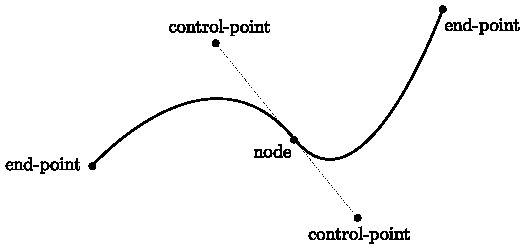
\includegraphics{../graphics/bezier.pdf}
\]
With the end points remaining fixed, the artist can move the node and
control points to change the way the curve looks.  But how do those
so-called control points actually control the way the curve looks?
Well, the end points, node, and control points define a polygonal path:
\[
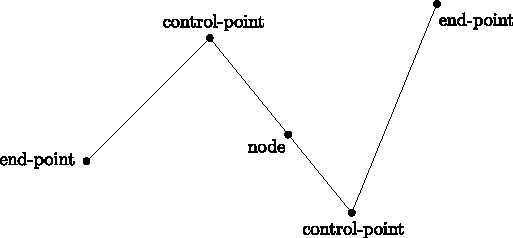
\includegraphics{../graphics/bezierPoly.pdf}
\]
This polygonal path in turn gives an envelope of tangents, which then gives
the desired curve:
\[
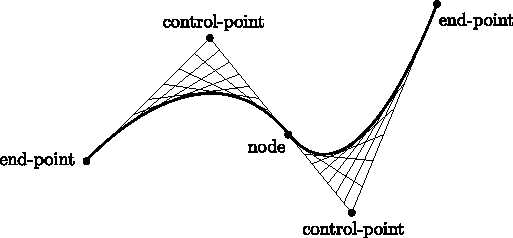
\includegraphics{../graphics/bezierMesh.pdf}
\]
While this may seem all fancy and highfalutin, it is the essence of
B\'ezier's method for drawing curves.  It has become so popular that
this is basically how curves are currently drafted using vector
graphics programs such as \textit{Adobe Illustrator} and
\textit{Inkscape}. Why are B\'ezier curves so popular? We'll see that
they satisfy the requirements above quite well.

\paragraph{Easy to Render}
A computer does not draw the parabola via an envelope of
tangents---however, the process we use above can be done by hand. The
key point is that one can obtain an arbitrary amount of smoothness to
the hand-drawn curve by simply adding  more lines to the envelope of tangents.



\paragraph{Easy to Transform}
Each curve is completely determined by the polygonal path from the
first end point to first control point to the node to the other
control point and the final end point. Hence, if I simply handed you
five points:
\[
(1,4)\to (4,2)\to (6,6)\to (7,8)\to(9,4)
\]
you can then draw a curve and tell someone else how to draw the exact
same curve. Moreover, if you take a geometric transformation like one
of the matrices we've studied, you could transform the entire
curve merely by transforming those five points.



\paragraph{Easy to Draft}
Of course, as you are aware, most graphic artists don't think much
about coordinates and yet are still able to draw B\'ezier curves with
impunity. This is really the genius of B\'ezier's method. By fixing
the end points, one only need to know the position of the node and the
control points. So by using a mouse, an artist can move the
control points and node to get a plethora of interesting curves.


\begin{ques}
What interesting pictures can \textit{you} make with B\'ezier curves?
\end{ques}
\QM

\newpage


\problems
\begin{enumerate}
\item Sketch the graph of $y= x^2$. On the same plot, draw a 7-line
  envelope of tangents defined by the line segments that go from
  $(2,4)$ to $(0,-4)$ and $(-2,4)$ to $(0,-4)$.
\item Sketch the graph of $y= x^2/8$. On the same plot, draw a 7-line
  envelope of tangents defined by the line segments that go from $(8,8)$
  to $(0,-8)$ and $(-8,8)$ to $(0,-8)$.
\item Use a 7-line envelope of tangents to approximate one quarter of a
  circle. Compare your drawing with an actual quarter of a
  circle. What do you notice?
\item Your client gives you the following rough sketch of an arched
  ceiling in a hallway:
\[
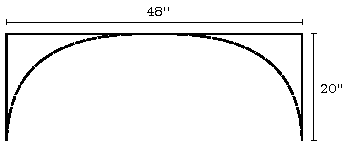
\includegraphics{../graphics/stringHall.pdf}
\]
Give an accurately scaled drawing of this arch, and explain how it can
be enlarged to actual size.
\item Your client gives you the following rough sketch of a lancet
  arch:
\[
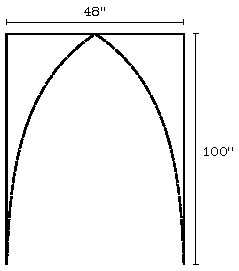
\includegraphics{../graphics/stringLancet.pdf}
\]
Use an envelope of tangents to give an accurately scaled drawing of this arch, and explain how it can
be enlarged to actual size.
\item Your client gives you the following rough sketch of a pointed
  arch. They would like the dotted triangle to be an equilateral
  triangle:
\[
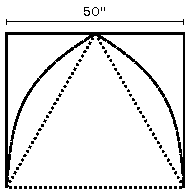
\includegraphics{../graphics/stringEquiArch.pdf}
\]
Use an envelope of tangents to give an accurately scaled drawing of
this arch, and explain how it can be enlarged to actual size.
\item Your client gives you the following rough sketch of a parabolic
  arch:
\[
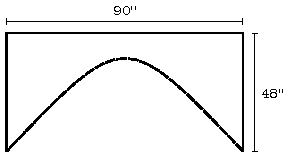
\includegraphics{../graphics/stringParaArch.pdf}
\]
Use an envelope of tangents to give an accurately scaled drawing of
this arch, and explain how it can be enlarged to actual size.
\item Your client gives you the following rough sketch of a round
  arch:
\[
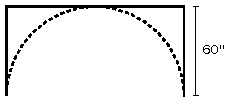
\includegraphics{../graphics/stringRoundArch.pdf}
\]
Give \textit{two} accurately scaled drawings of this arch: One given
by envelope of tangents, and one that is actually semi-circular. In
both cases, explain how your drawings can be enlarged to actual size.


\item Suppose you draw an envelope of tangents by continually taking
  midpoints as we did above. This will form a 1-line envelope of tangents,
  then a 3-line envelope of tangents, then a 7-line envelope of tangents, then
  a 15-line envelope of tangents, and so on. What is the pattern? Explain
  why the pattern holds.


\item Concerning B\'ezier curves: why are the control points and node
  always on a straight line?  What would happen if they weren't?
\item The following five points determine a polygonal path:
\[
(1,4)\to (4,2)\to (6,6)\to (7,8)\to (9,4)
\]
Using a 7-line envelope of tangents, draw the corresponding B\'ezier curve.
\item The following five points determine a polygonal path:
\[
(1,2)\to (2,7)\to (4,6)\to (8,4)\to (9,7)
\]
Using a 7-line envelope of tangents, draw the corresponding B\'ezier curve.
\item The following five points determine a polygonal path:
\[
(4,2)\to (1,6)\to (4,6)\to (6,6)\to (8,9)
\]
Using a 7-line envelope of tangents, draw the corresponding B\'ezier curve.
\item The following five points determine a polygonal path:
\[
(1,5)\to (4,2)\to (6,6)\to (7,8)\to (6,1)
\]
Using a 7-line envelope of tangents, draw the corresponding B\'ezier curve.
\item The following five points determine a polygonal path:
\[
(3,1)\to (1,6)\to (5,7)\to (9,8)\to (8,3)
\]
Using a 7-line envelope of tangents, draw the corresponding B\'ezier curve.
\item Your client gives you the following rough sketch of a horseshoe
  arch:
\[
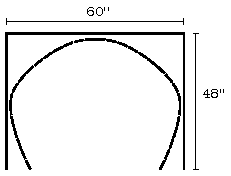
\includegraphics{../graphics/stringHorseShoe.pdf}
\]
Use an envelope of tangents to give an accurately scaled drawing of
this arch, and explain how it can be enlarged to actual size.
\item Compare the two polygonal paths:
\begin{align*}
&(1,2)\to (2,7)\to (4,6)\to (8,4)\to (9,7)\\
&(1,2)\to (8,4)\to (4,6)\to (2,7)\to (9,7)
\end{align*}
Using a 7-line envelope of tangents, draw the corresponding B\'ezier
curve for each. What does this tell you about the order of the points
in the polygonal-path?
\item In the examples of polygonal paths we've given you so far
\[
\vec{a} \to \vec{b} \to \vec{c} \to \vec{d} \to \vec{e}
\]
the points $\vec{b}$, $\vec{c}$, and $\vec{d}$ have all been on a
line. What will happen if they are not on a line? Explain your
reasoning.

\item The following points determine a polygonal path:
\[
(8,0)\to (0,0)\to (0,8)
\]
\begin{enumerate}
\item Draw the corresponding 7-line envelope of tangents. 
\item Apply the matrices
\[
\mat{R}_{90}, \qquad \mat{R}_{90}^2, \qquad \mat{R}_{90}^3
\]
to your points. Then in each case, draw the corresponding 7-line
envelope of tangents. 
\end{enumerate}
Show all your work.

\item The following points determine a polygonal path:
\[
(8,0)\to (8,8)\to (0,8)
\]
\begin{enumerate}
\item Draw the corresponding 7-line envelope of tangents. 
\item Apply the matrices
\[
\mat{R}_{90}, \qquad \mat{R}_{90}^2, \qquad \mat{R}_{90}^3
\]
to your points.  Then in each case, draw the corresponding 7-line
envelope of tangents. 
\end{enumerate}
Show all your work.

\item The following points determine a polygonal path:
\[
(-4,-4) \to (0,-4)\to (0,0)\to (0,4)\to (4,4)
\]
\begin{enumerate}
\item Using a $7$-line envelope of tangents, draw the corresponding B\'ezier
curve. 
\item Apply the matrices
\[
\mat{R}_{90}, \qquad \mat{R}_{90}^2, \qquad \mat{R}_{90}^3
\]
to your points.  Then in each case, draw the corresponding 7-line
envelope of tangents.
\end{enumerate}
Show all your work.

\end{enumerate}
